\section{Comparación}

Para poder ilustrar mejor las diferencias entre las imágenes originales y las comprimidas, tanto en escala de grises como en color, se creó un notebook de Jupyter que presenta los resultados visuales. Esta notebook fue generada con apoyo de herramientas con inteligencia artificial y cumple únicamente el propósito de demostración gráfico y no afecta directamente en el desarrollo técnico de proyecto.

\subsection{Imagenes de comparación}

\begin{figure}[htbp]
  \centering
  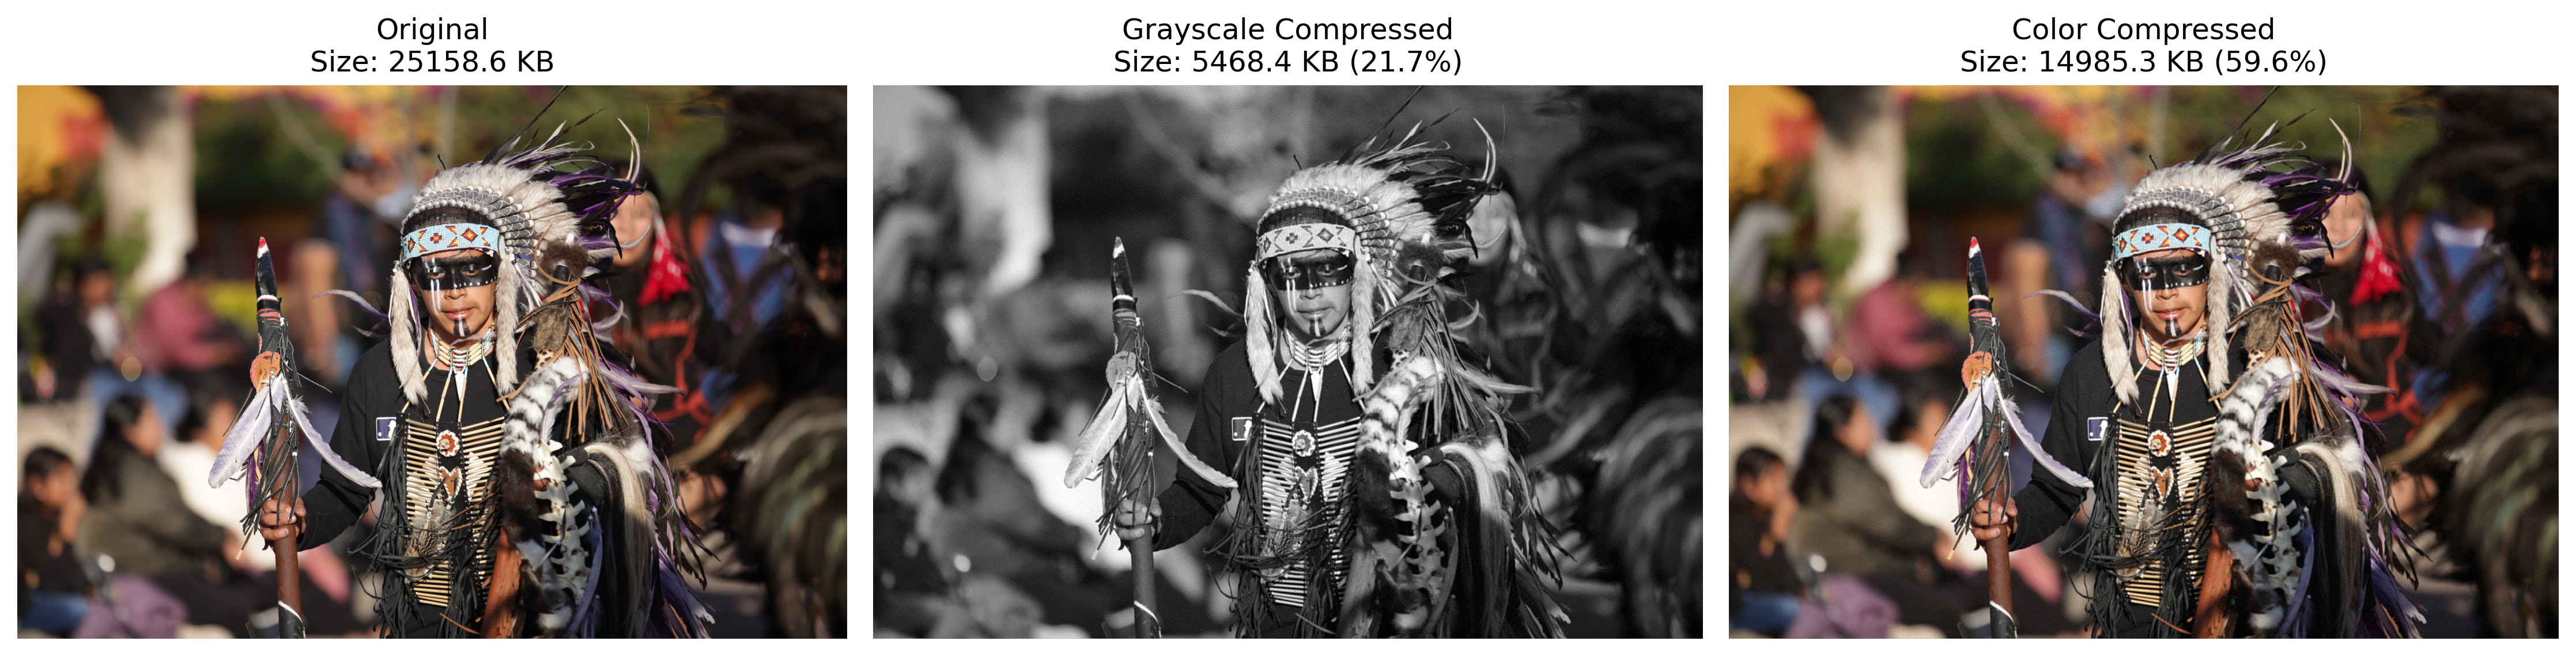
\includegraphics[width=0.8\textwidth]{sources/comparison/test_1.png}
  \caption{Resultados de compresión imagen 1}\label{fig:comparison1}
\end{figure}

\begin{figure}[htbp]
  \centering
  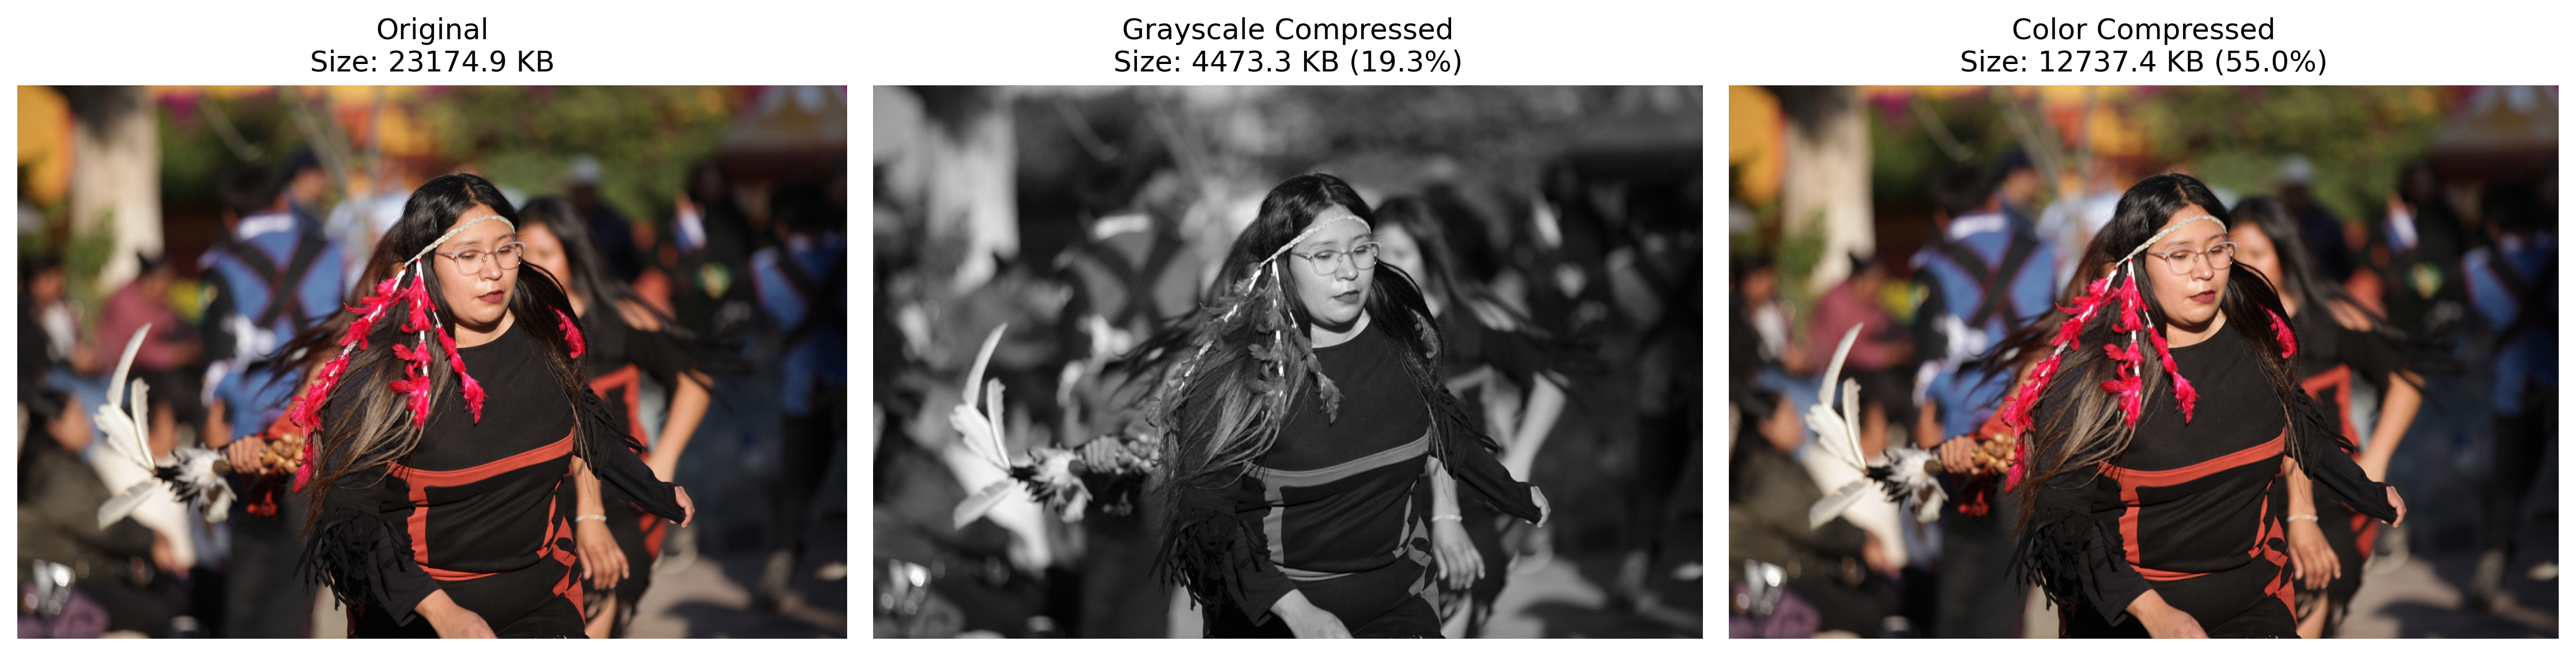
\includegraphics[width=0.8\textwidth]{sources/comparison/test_2.png}
  \caption{Resultados de compresión imagen 2}\label{fig:comparison2}
\end{figure}

\begin{figure}[htbp]
  \centering
  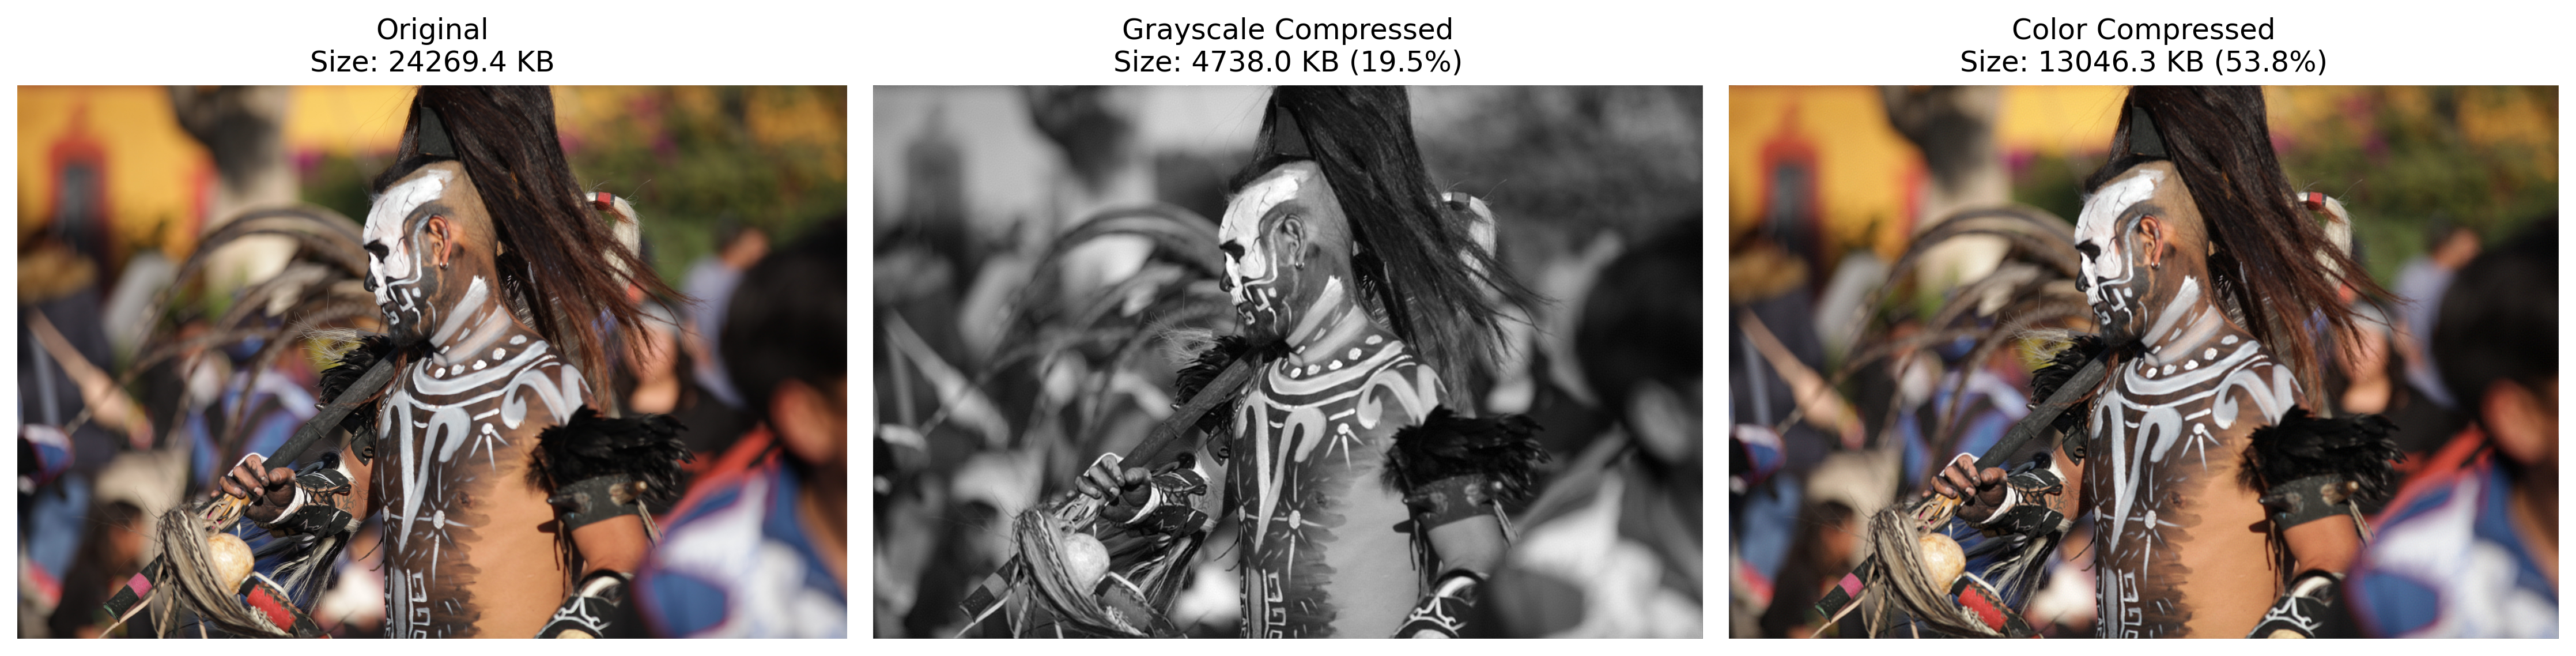
\includegraphics[width=0.8\textwidth]{sources/comparison/test_3.png}
  \caption{Resultados de compresión imagen 3}\label{fig:comparison3}
\end{figure}

\subsection{Observaciones sobre las imagenes}

Con la implementación del método basado en FFT 2D se logró reducir el tamaño de los archivos sin sacrificar visualmente los detalles esenciales. Al transformar las imágenes se mantiene intacta una estructura general, contornos, gradaciones suaves y las texturas continuas.

Para las imágenes de color, el método FFT 2D logra reducir las imágenes entre un 50\% y un 60\% de su tamaño original. Esto se debe a que los 3 canales de color (rojo, verde y azul) comparten redundancias y el FFT 2D logra descartar muchas frecuencias sin que aparezca perceptibles.

Para las imágenes en escala de grises se puede observar que la compresión es menor, se logra reducir entre un 15\% y un 25\%, lo cual sigue siendo un tamaño considerable.

Visualmente se puede observar que las imágenes son perfectamente perceptibles. Al ampliar la imagen comprimida, se puede percibir una ligera cantidad de ruido y algunos bordes ligeramente más duros, pero cumple con la función de compresión.

Es importante destacar que aunque la compresión es consistente en la mayor parte de los casos, aunque si existe la posibilidad de que la imagen no se comprima adecuadamente si esta contiene muchos detalles granulares o ruido visual (como partículas).